\let\negmedspace\undefined
\let\negthickspace\undefined
\documentclass[journal]{IEEEtran}
\usepackage[a5paper, margin=10mm, onecolumn]{geometry}
\usepackage{lmodern} % Ensure lmodern is loaded for pdflatex
\usepackage{tfrupee} % Include tfrupee package

\setlength{\headheight}{1cm} % Set the height of the header box
\setlength{\headsep}{0mm}     % Set the distance between the header box and the top of the text

\usepackage{gvv-book}
\usepackage{gvv}
\usepackage{cite}
\usepackage{amsmath,amssymb,amsfonts,amsthm}
\usepackage{algorithmic}
\usepackage{graphicx}
\usepackage{textcomp}
\usepackage{xcolor}
\usepackage{txfonts}
\usepackage{listings}
\usepackage{enumitem}
\usepackage{mathtools}
\usepackage{gensymb}
\usepackage{comment}
\usepackage[breaklinks=true]{hyperref}
\usepackage{tkz-euclide} 
\usepackage{listings}                                      
\def\inputGnumericTable{}                                 
\usepackage[latin1]{inputenc}                                
\usepackage{color}                                            
\usepackage{array}                                            
\usepackage{longtable}
\usepackage{multicol}
\usepackage{calc}                                             
\usepackage{multirow}                                         
\usepackage{hhline}                                           
\usepackage{ifthen}                                           
\usepackage{lscape}
\begin{document}

\bibliographystyle{IEEEtran}
\vspace{3cm}

\title{12.9.2.2}
\author{EE24BTECH11010 - Balaji B}
% \maketitle
% \newpage
% \bigskip
{\let\newpage\relax\maketitle}

\renewcommand{\thefigure}{\theenumi}
\renewcommand{\thetable}{\theenumi}
\setlength{\intextsep}{10pt} % Space between text and floats


\numberwithin{equation}{enumi}
\numberwithin{figure}{enumi}
\renewcommand{\thetable}{\theenumi}


\textbf{Question}:\\
Solve the differential equation $y^{\prime}-2x-2 = 0$ with initial conditions $y\brak{0} = 0$

\textbf{Theoretical Solution:}\\
We apply the Laplace transform to each term in the equation. The Laplace transforms for the derivatives of $y\brak{x}$ are:
\begin{align}
\mathcal{L}\cbrak{y^{\prime}\brak{x}} &= sY\brak{s} - y\brak{0} \\
\mathcal{L}\cbrak{2x} &= 2 \cdot \frac{1!}{s^2} = \frac{2}{s^2}, \\
\mathcal{L}\cbrak{2} &= \frac{2}{s}.
\end{align}
Now, applying the Laplace transform to the entire differential equation:
\begin{align}
\mathcal{L}\cbrak{y^{\prime}-2x-2} &= 0\\
\mathcal{L}\cbrak{y^{\prime}\brak{x}} - \mathcal{L}\cbrak{2x} - \mathcal{L}\cbrak{2} &= 0 \\
sY\brak{s} - y\brak{0} - \frac{2}{s^2} - \frac{2}{s} &= 0
\end{align}
Substitute the initial conditions $y\brak{0} = 0$, we get
\begin{align}
sY\brak{s} - 0 - \frac{2}{s^2} - \frac{2}{s} &= 0
\end{align}
Simplify the equation:
\begin{align}
    sY(s) =  \frac{2}{s^2} + \frac{2}{s}\\
    Y(s) =  \frac{2}{s^3} + \frac{2}{s^2}
\end{align}
Now, take the inverse Laplace transform \\
\begin{align}
y(x) &= \mathcal{L}^{-1}\cbrak{Y(s)}\\
y(x) &=   \mathcal{L}^{-1}\cbrak{\frac{2}{s^3}} + \mathcal{L}^{-1}\cbrak{\frac{2}{s^2}}\\
y(x) &=  2x + x^2
\end{align}
Region of Convergence:\\
The denominator indicates a pole at $s= 0 $. To ensure convergence of the Laplace transform integral, the real part of $s$ must satisfy:
\begin{align}
    Re\brak{s}>0
\end{align}
So the Laplace transform converges for values of $s$ with real part greater than 0\\

\textbf{Computational Solution: }\\ \\
The \textbf{ bilinear transform} is used to approximate the continuous derivative $y^{\prime}$ and reformulate the differential equation into a discrete time difference equation.\\
Applying the Laplace transform to both sides of the differential equation, we get
\begin{align}
sY\brak{s} - 0 - \frac{2}{s^2} - \frac{2}{s} &= 0\\
sY(s) =  \frac{2}{s^2} + \frac{2}{s}\\
Y(s) =  \frac{2}{s^3} + \frac{2}{s^2}
\end{align}
Apply Bilinear Transform with $T=h$
\begin{align}
    s&=\frac{2}{T}\frac{1-z^{-1}}{1+z^{-1}}
\end{align}
Substituting the above in our Laplace equation we get,
\begin{align}
    Y(z) &= \frac{2}{\brak{\frac{2}{T}\frac{1-z^{-1}}{1+z^{-1}}}^3} + \frac{2}{\brak{\frac{2}{T}\frac{1-z^{-1}}{1+z^{-1}}}^2} \\ 
    Y(z) &= \frac{2}{\brak{\frac{2}{h}\frac{1-z^{-1}}{1+z^{-1}}}^3} + \frac{2}{\brak{\frac{2}{h}\frac{1-z^{-1}}{1+z^{-1}}}^2}
\end{align}
On rearranging and neglecting the powers greater than 2 of $h$ we get,
\begin{align}
    (1 - z^{-1})^3Y(z) &= \frac{h^2\brak{1 - z^{-2}}\brak{1 + z^{-1}}}{2} \\
    \brak{1 - 3z^{-1} + 3z^{-2} - z^{-3}}Y(z) &= \frac{h^2\brak{1 + z^{-1} - z^{-2} - z^{-3}}}{2}
\end{align}
Applying $Z$ transform we get
\begin{align}
    y_n - 3y_{n-1} + 3y_{n-2} - y_{n-3} &= \frac{h^2 \brak{\delta\sbrak{n}+\delta\sbrak{n-1}-\delta\sbrak{n-2}-\delta\sbrak{n-3}}}{2}
\end{align}
\\The above equation is the required difference equation.\\ \\
Taking the value of $h$ = 0.1, we get the following plot

\begin{figure}[h!]
   \centering
   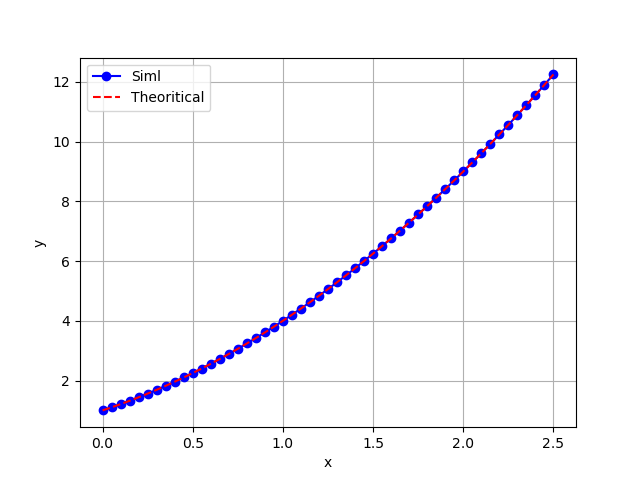
\includegraphics[width=0.7\columnwidth]{figs/fig.png}
    \caption{Approximate solution of the DE}
\end{figure}
\end{document}
